% !TEX root = ../thesis.tex

\chapter{绪论}
\section{引言}
	在实际工程应用中,由于种种因素,如信息传输丢失、外部环境突变、子系统连接变化等,可能会导致系统结构、参数的变化。为了描述这种现象,学者们提出了Markov模型来对这类系统进行建模,并称这类系统为Markov跳变系统。近年来,由于Markov跳变系统对上述现象的强大建模能力获得了广泛而深入的研究。同时,非线性是控制系统中最常见的一类现象,在众多的非线性类别中,有一种非线性因其广泛存在及独特的性质,学者们对其进行了专门而系统的研究,并称之为Lur'e系统。由于一些应用使用一维(1D)系统模型难以建模或模型不够精确,因而学者们提出了能更加精确建模的二维(2D)控制系统模型。在本文中,我们将围绕Markov跳变Lur'e系统、2D-Markov跳变系统展开讨论。在本章,我们重点介绍Markov跳变系统及研究现状,给出阅读本文需要的预备知识背景并介绍本文的研究内容。至于Lur'e系统、2D系统以及相关的控制概念,我们将在稍后的相关章节中作进一步的详细介绍。

\section{Markov跳变系统}
	Markov跳变系统实际上是一种特殊的切换系统,当系统的结构、参数发生变化时,我们认为系统由某个子系统切换到了另一个子系统,同时,我们使用模态来表示这若干个子系统。根据这样的假设,不难发现,系统有多少种不同的结构、参数,就应该有多少个子系统,对应同等数量的系统模态。同其他切换系统不同的是,Markov跳变系统模态之间的切换是由一个Markov链来控制的,即模态切换遵循Markov过程。一个简单的离散Markov跳变系统\eqref{intro-system-eq}可以表示为,
	\begin{equation}\label{intro-system-eq}
		x(k+1)=A(r(k))x(k)+B(r(k))u(k)
	\end{equation}
	这里$\{r(k),k\geq 0 \}$表示系统模态对应的Markov链,$N$表示系统的模态总数。人们通过对系统模态进行统计,得到模态间的切换规律,并将其表示为具有如下形式的模态转移概率
	\begin{equation}\label{introduction-tps-sys}
	\Pr\{r(k+1)=j|r(k)=i \}=\pi_{ij}
	\end{equation}
	因此,一般来说,系统在下一个时刻的模态可以由当前模态通过模态转移概率推测得到。一个简单具有$N$个模态的Markov跳变系统可以用图\ref{intro_system}表示。
	\begin{figure}[!htb] 
		\centering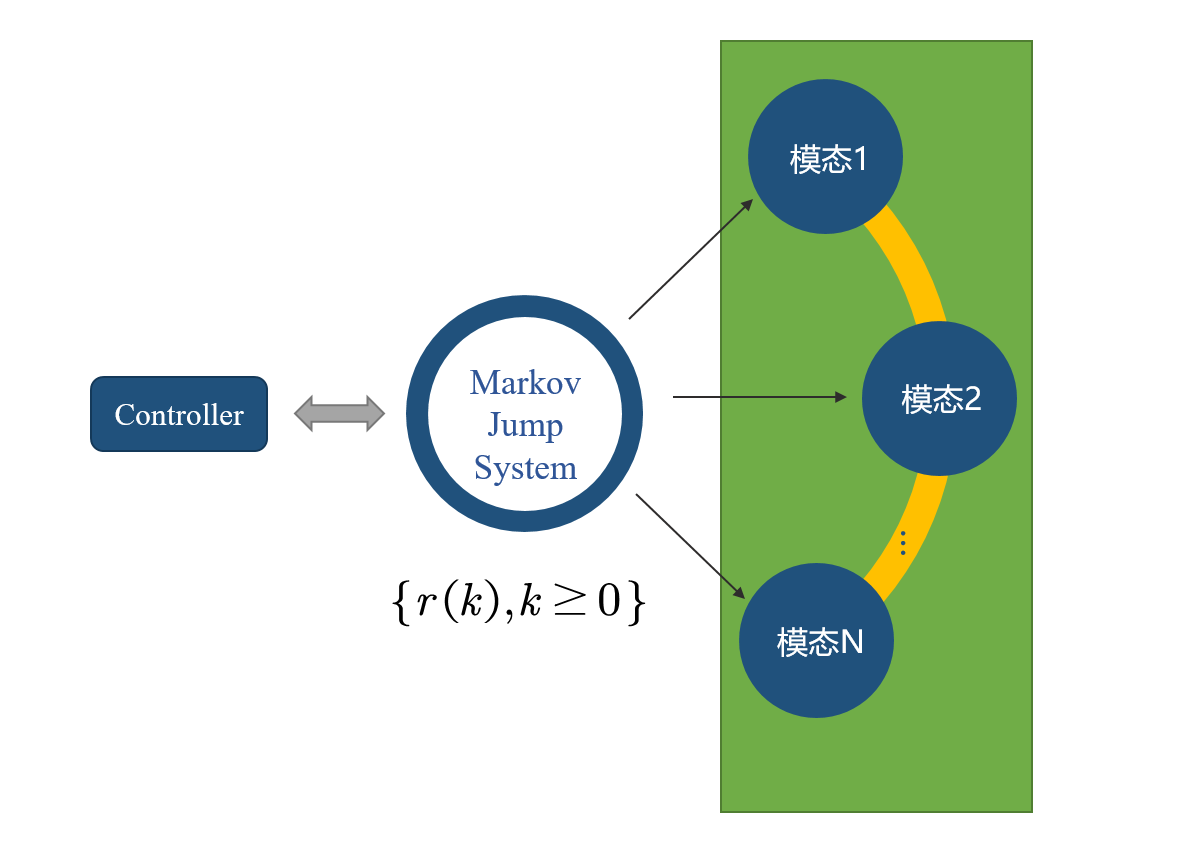
\includegraphics[scale=0.25]{./figures/introduction/system.png}\\ 
		\caption{Markov跳变系统示意图}
		\label{intro_system}
	\end{figure}

	自Markov跳变系统首次提出以来\cite{florentin1961optimal},便取得了国内外学者们的广泛关注,并取得了众多理论研究成果\cite{costa2006discrete,de2000output,xiong2005robust,ma2010stability,zhang2009hestimation,xu2007delay}。同时,Markov跳变控制系统已经成功的应用到诸如,金融分析系统\cite{mamon2007hidden}, 故障检测\cite{zhong2005faultdetection},网络通讯\cite{network-communication-kim2004},飞行器控制\cite{bar1993estimation,gray2000stability},机器臂\cite{goncalves2004nonlinear}等实际应用中。近年来,Markov跳变系统取得了诸多突破性的进展。例如,针对模态转移概率可能不确定的情况,文献\cite{zhang2009stability}提出了系统模态转移概率部分已知的控制方法,该方法涵盖了模态转移矩阵完全已知、完全未知的情况,并且利用该方法对连续、离散线性Markov跳变系统的稳定性进行了分析。之后,一些学者将该方法分别推广到了$H_{\infty}$控制\cite{luan2012h},$H_\infty$滤波\cite{ma2009robust},奇异系统\cite{kao2014stabilization}等。

\section{模态信息不匹配控制}
	目前,就Markov跳变系统,根据控制器模态同系统模态的匹配情况,可以将控制器分为三类:模态独立控制器、模态同步控制器、异步控制器。下面我们将针对这三类控制器分别展开讨论。
	\subsection{同步控制器}
	同步控制器对应的是模态信息完全匹配的情况,一般来说,系统应该有如下形式,
	\begin{equation}
		u(k)=K(r(k))x(k)
	\end{equation}
	这里,不难发现,控制器的模态和系统的模态都是使用$r(k)$来表示的,也就是说,控制器的模态应该同系统模态保持一致,即控制器模态同系统模态完全匹配。最早关于Markov跳变系统的研究都假设控制器的模态是和系统模态保持一致的,并且取得了众多的研究成果。一般而言,模态完全匹配的情况,在系统分析上比较简单,同时,得到的结果也会比其他两种情况要好一些。但是,在实际控制系统中,控制器模态想要同系统模态始终保持一致是非常困难的。首先,由于在网络传输过程中存在信息丢失的情况,控制器可能在某些时刻获取不到系统模态信息。其次,由于网络传输存在延迟,控制器可能得到的是先前时刻的系统模态信息,而此时系统已经切换到另外一个模态,进而导致控制器模态同系统模态不匹配。另外,即使控制器及时的得到了当前时刻精确的系统模态信息,但是由于物理因素的限制,控制器可能不能及时的切换到对应模态,即控制器模态切换速度跟不上系统模态切换速度,进而又出现了模态不匹配的情况。就是说,如果想要实现模态信息始终匹配,我们需要拥有一套先进的信息传输、物理切换装置,显然,目前的科技水平是很难达到的。因此,同步控制器设计尽管分析起来非常简单,却有些不太符合实际情况了。
	
	\subsection{模态独立控制器}
	模态独立控制器对应的是模态信息完全不匹配的情况,一般来说,系统应该有如下形式,
	\begin{equation}
	u(k)=K(q(k))x(k)
	\end{equation}
	这里,$q(k)$表示控制器在$k$时刻的模态,可能在集合$\{1,2,\dots,M \}$中取值,但是服从另外一个独立的Markov过程,其状态转移概率为
	\begin{equation}\label{introdution-tps-indp}
	\Pr\{q(k+1)=j|q(k)=i \}=\lambda_{ij}
	\end{equation}
	由\eqref{introdution-tps-indp}可以推断,对模态独立控制器的情况,当前时刻的控制器模态只跟上一个时刻的控制器模态有关,同系统模态没有任何关系,即控制器模态同系统模态完全不匹配(注意,本文中,完全不匹配并不是指控制器模态始终同系统模不一致,而是两者之间不存在联系的意思)。图\ref{intro_fig_idpsys}表示了一个简单的模态独立控制器作用下的Markov跳变系统。目前,文献\cite{todorov2016new,wu2005mode,dolgov2017static}对模态独立Markov控制问题展开了研究,并得到了相应的结果。值得注意的是,当我们施加了$M=N$,$\lambda_{ij}=\pi_{ij}$,$r(0)=p(0)$这三个限制条件后,似乎控制器变成了模态完全匹配(同步)的情况,但本质上却并不是同步控制器。一个简单的理解为,假设$k$时刻系统模态和控制器模态是一样的,但是由于控制器和系统在$k+1$时刻的模态都是由概率(此时概率一样)求得的,因此也可能模态不一致,而同步控制器里,控制器在$k+1$时刻的模态是通过检测$k+1$时刻系统模态得到的。对于模态独立控制器,我们发现控制器完全没有使用到系统的模态信息,这可能导致的结果就是,最终得到的结果会比较保守,同时,在系统分析时也相对比较困难。
	
	\begin{figure}[!htb] 
		\centering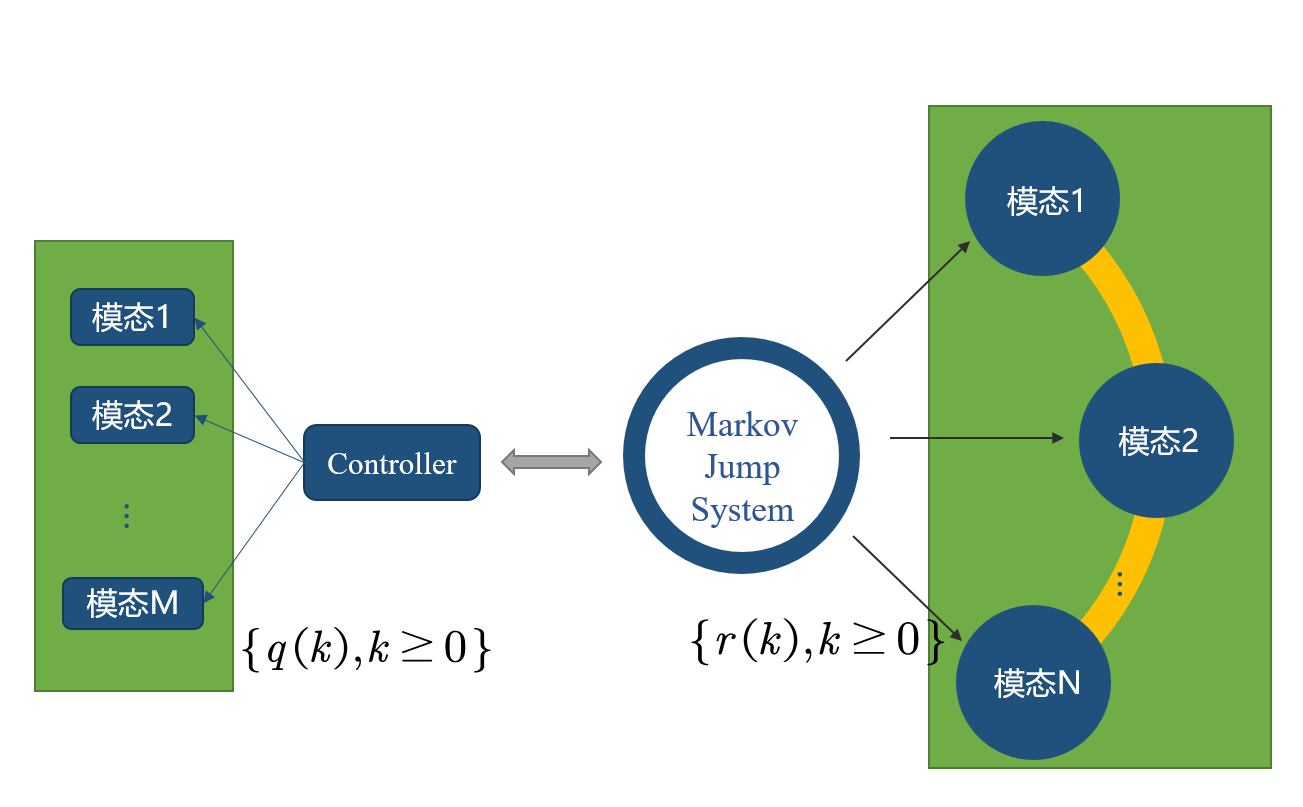
\includegraphics[scale=0.25]{./figures/introduction/idpsys.png}\\ 
		\caption{模态独立控制器作用下的Markov跳变系统}
		\label{intro_fig_idpsys}
	\end{figure}
	
	\subsection{异步控制器}
	模态独立控制器对应的是模态信息不完全匹配的情况,一般来说,系统应该有如下形式,
	\begin{equation}
	u(k)=K(\sigma(k))x(k)
	\end{equation}
	这里,$\sigma(k)$表示控制器在$k$时刻的模态,可能在集合$\{1,2,\dots,M\}$中取值,服从一个满足如下条件模态转移概率的从随机跳变过程,
	\begin{equation}\label{introdution-tps-asyn}
	\Pr\{\sigma(k)=\phi|r(k)=i \}=\mu_{i\phi}
	\end{equation}
	由\eqref{introdution-tps-asyn}我们可以发现,控制器在$k$时刻的模态是由$k$时刻的系统模态和条件概率求得的。对比同步控制器,我们可以理解同步控制器为$\mu_{ii=1}$的情况。也就是说,对同步控制器而言,$k$时刻系统模态是多少,控制器的模态就应该是多少,而对异步控制器而言,$k$时刻控制器的模态却是通过条件概率求得的,并不一定同系统模态保持一致。对比模态独立控制器,$k$时刻模态独立控制器的模态是由前一时刻($k-1$)推测的,根本就没有利用任何时刻系统的模态信息。那么,我们发现,下面几个结论(异步控制器的优点)
		
		(1) 异步控制器通过调整条件概率转变成同步控制器,
		
		(2) 异步控制器不需要严格要求控制器模态同系统模态保持一致,更符合实际情况,
		
		(3) 同模态独立控制器相比,异步控制器利用了更充分的系统信息,得到的结果更加有价值。
		
		结论(1)是比较直观的。我们重点讨论一下结论(2),这里需要注意的是,相对于同步控制器,异步控制器削弱了对同步控制器三个完美前提的依赖, 即:一定能获得系统的模态信息、系统模态信息获得足够及时、控制器在获得系统模态信息后能马上切换。异步控制器,对于上述三个前提假设,并没有采用什么优秀的改进方法来改善它们,而是正视这些不完美的存在。控制器通过一个检测器预先采集足够多的信息,统计模态间的切换规律,来推断当前控制器所处的模态。因此,在许多文章中,又称异步控制器设计方法为基于检测器的控制器设计方法。另一方面,前文中已经说过,异步控制器是基于隐Markov模型设计的,因此,基于隐Markov模型设计的控制器可以涵盖同步、异步、模态独立(1个模态)这三种情况,是一个比较综合的控制器设计方法。
		
		由上述可知,基于隐Markov模型的异步控制器在处理模态不匹配的场景下具有诸多优势。因此,在本文中,我们将采用该模型来设计异步控制器,进而对系统的稳定性及各种性能进行分析。
	
	\begin{figure}[!htb] 
		\centering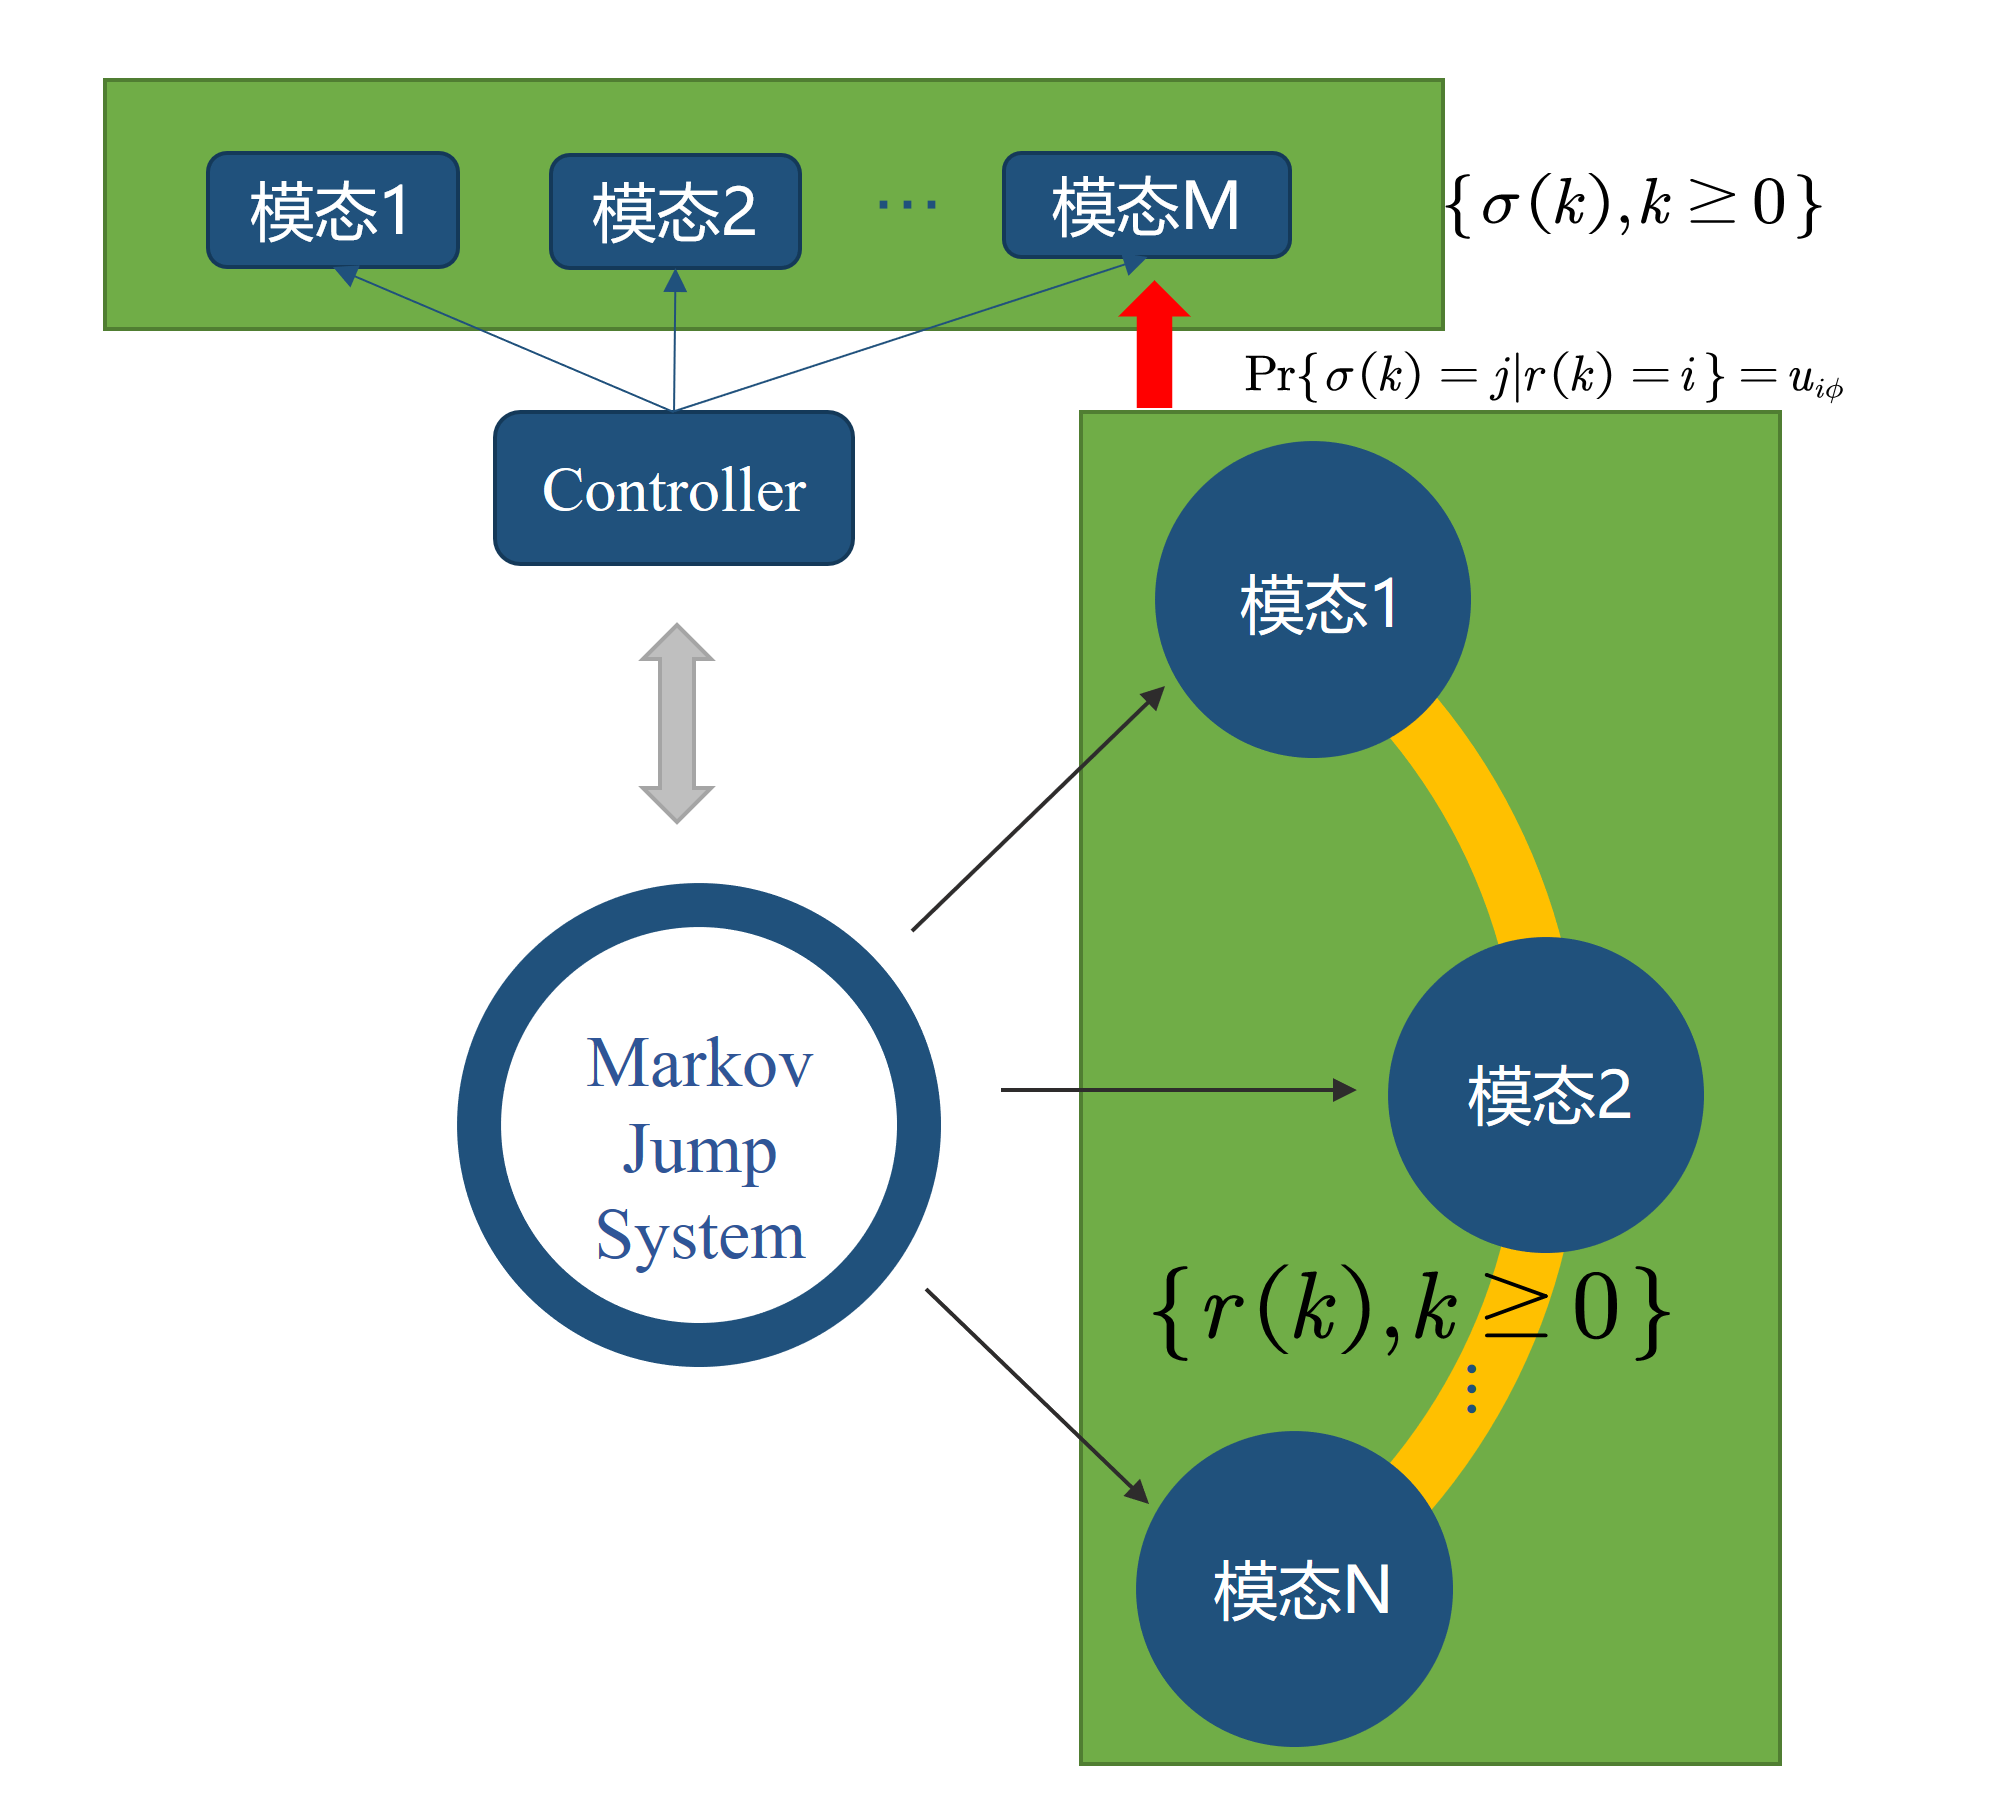
\includegraphics[scale=0.12]{./figures/introduction/asynsys.png}\\ 
		\caption{异步控制器作用下的Markov跳变系统}
		\label{intro_fig_asynsys}
	\end{figure}
	
\section{预备定理}
	本文中,我们将尽量将最终结果以LMI的形式呈现,因此需要使用到Schur补引理将普通的非线性不等式转换为LMI。
	
	{\bf 引理 \ \ 1.1:}(Schur补引理\cite{boyd1994linear}) 给定矩阵实对称矩阵$S_{11}\in\mathbb{R}^{n\times n}$,$S_{22}\in\mathbb{R}^{m\times m}$,矩阵$S_{12}\in\mathbb{R}^{n\times m}$,则下面三个条件是等价的
	\begin{equation}
		\begin{bmatrix}
			S_{11}&S_{12}\\
			*&S_{22}
		\end{bmatrix}<0,
	\end{equation} 
	\begin{equation}
		S_{11}<0,S_{22}-S^{T}_{12}S^{-1}_{11}S_{12}<0,
	\end{equation} 
	\begin{equation}
		S_{22}<0,S_{11}-S^{T}_{12}S^{-1}_{22}S^{T}_{12}<0.
	\end{equation} 
		
\section{本文的研究内容}
	由于诸如信息传输丢失、外部环境突变、子系统连接变化等因素的影响,会导致系统结构、参数的突变,学者们使用Markov系统来对这类现象进行建模,并在过去的几十年里取得了许多重要的成果。另一方面,非线性广泛的存在实际控制系统中,因此非线性Markov跳变系统也是一种非常重要的控制系统。目前大多数对非线性Markov跳变系统的研究都基于控制器模态同系统模态这一严格的假设,但是由于这一假设对通讯、切换等物理装置的要求过于严格,因此尽管取得的成果非常优秀,却很难实现,因此并不能在实际应用中进行广泛推广。隐Markov模型削弱了该假设的严格要求,同时充分利用了系统信息,是一个优秀的包含模态完全匹配、模态部分匹配、模态完全不匹配的统一模型。本文中将基于隐Markov模型来设计异步控制器,对非线性Markov跳变系统的稳定性,$l_2$、$H_\infty$、保成本等性能进行研究。具体的工作主要归纳如下:
	
	(1) 在第二章中,考虑到Lur'e系统在实际应用中的普遍性、在非线性系统中的重要地位,我们对一类Markov跳变Lur'e系统展开了研究。首先考虑到控制器模态同系统模态可能存在不匹配的情况,因此我们引入了隐Markov模型来设计异步控制器;该控制器由一个线性状态反馈和一个非线性输出反馈组成,这个非线性环节同Lur'e系统的非线性是一样的,都满足一个有限扇形条件,这样的控制器结构可以使得我们得到的结果相比只有状态反馈的结构得到的结果更加不保守;随后,我们对这类Markov跳变Lur'e系统的稳定性及$l_2$性能进行了研究,得到了满足一定$l_2$性能同时保证系统随机稳定的充分条件。最后,我们使用了一个例子验证了异步控制器的有效性,同时探究了条件转移概率、控制器异步率、最优$l_2$性能之间的关系。
	
	(2) 在第三章中,我们研究了一类Rosser模型下的非线性二维Markov跳变控制系统的滑模控制问题。考虑到2D系统的特殊结构给系统分析先比1D系统带来了更多的复杂性和困难,我们构造了一个新颖的2D滑模面。同时考虑到控制器模态同系统模态的不匹配情况,基于构造的滑模面,引入了隐Markov模型设计了一个2D异步滑模控制器。我们首先研究了在此异步滑模控制器下系统的稳定性及$H_\infty$性能问题,得到了能够使得系统满足一定$H_\infty$性能同时保证渐进均方稳定的充分条件;同时,我们又研究了系统状态到滑模面的可达性问题,得到了一个可以使得系统状态到达滑模面某个领域内部的充分条件;然后,我们在上述两个结果的基础上,给出了能够保证一定$H_\infty$性能且稳定的同时,保证系统状态可达性的充分条件。随后,我们把本章结果进行归纳,得到了一个2D异步滑模控制器设计算法。最后,我们使用了一个数值仿真例子来验证2D异步滑模控制的有效性。
	
	(3) 在第三章中,我们研究了Rosserm模型下二维Markov跳变系统的二次型控制问题。首先,考虑到控制器模态同系统模态的不匹配问题,基于隐Markov模型,我们设计了一个异步线性状态反馈控制器。同时,定义了一个二次型成本函数,并分别讨论了三种不同的初始条件下系统的稳定性和保成本性能问题。相对1D系统,由于2D系统的初始模态和初始状态都不止一个,因此,情况也要更加的复杂,分析起来也更加困难。在本章中,我们把初始条件分为了三类进行讨论。第一种情况是假设初始模态和初始状态都已知,这种情况下,我们对系统的初始信息要求掌握的足够多,但是得到的保成本性能是最好的;第二种情况是假设初始模态已知,全部的初始状态都满足一定的约束条件,此时,我们简化了对系统初始状态的要求,但是保成本性能略有下降;第三种情况是系统的初始模态不知道,全部的初始状态满足一定的约束条件,在第二种情况的基础上进一步降低了对系统初始模态的要求,得到的结果形式是最为简单的,但是保成本性能也是三者里最差的。同时,不管是上述哪一种情况,我们都可以使用同一个条件来保证系统的稳定性。最后,我们同样使用了一个仿真实例来验控制器对系统的影响。
	
	
	
	
	
	